\documentclass[10pt,a4paper]{article}
\usepackage[T1]{fontenc}
\usepackage[scaled]{helvet}
\usepackage{cite}
\usepackage{url}
\usepackage{graphicx}
\usepackage{listings}
\usepackage{float}
\usepackage{amsmath}
\usepackage{listings}
\usepackage{color}
 
\definecolor{dkgreen}{rgb}{0,0.6,0}
\definecolor{gray}{rgb}{0.5,0.5,0.5}
\definecolor{mauve}{rgb}{0.58,0,0.82}
\lstset{ %
  language=Octave,                % the language of the code
  basicstyle=\footnotesize,           % the size of the fonts that are used for the code
  numbers=left,                   % where to put the line-numbers
  numberstyle=\tiny\color{gray},  % the style that is used for the line-numbers
  stepnumber=1,                   % the step between two line-numbers. If it's 1, each line 
                                  % will be numbered
  numbersep=5pt,                  % how far the line-numbers are from the code
  backgroundcolor=\color{white},      % choose the background color. You must add \usepackage{color}
  showspaces=false,               % show spaces adding particular underscores
  showstringspaces=true,         % underline spaces within strings
  showtabs=false,                 % show tabs within strings adding particular underscores
  frame=none,                   % adds a frame around the code
  rulecolor=\color{black},        % if not set, the frame-color may be changed on line-breaks within not-black text (e.g. commens (green here))
  tabsize=2,                      % sets default tabsize to 2 spaces
  breaklines=true,                % sets automatic line breaking
  breakatwhitespace=false,        % sets if automatic breaks should only happen at whitespace
  keywordstyle=\color{blue},          % keyword style
  commentstyle=\color{dkgreen},       % comment style
  stringstyle=\color{mauve},         % string literal style
  escapeinside={\%*}{*)},            % if you want to add LaTeX within your code
  morekeywords={*,...}               % if you want to add more keywords to the set
}
\usepackage{amssymb}
\usepackage{fancyhdr}
\usepackage{lastpage}
\floatstyle{boxed} 
\restylefloat{figure}
\renewcommand*\familydefault{\sfdefault}
\title{Threads and CPU Scheduling}
\author{David Lynch - david.lynch@raglansoftware.com }
\begin{document}
\maketitle
\begin{abstract}
In this article we will look at common algorithms that CPU schedulers implement. You'll find that these algorithms are relevant to other areas in which queues exist and decisions are made, so a clear understanding of the theory and implementation of these is essential. Firstly, we will talk about threads, which are a very important means for a process to execute internal function concurrently. 
\end{abstract}
\section{Threads}
Up to now we have considered process as an entity that will execute a single program in a {\bf single thread of control}. This means that internally, the process will execute only one code path concurrently. Separately, these single threaded processes will run concurrently with other processes. However, there are major advantages of facilitating concurrency within a process. A {\bf multi-threaded} application can run several code paths concurrently within a process. The advantage of being within the process is that there is seamless sharing of code, external resources such as files and a shared memory area. Coupled with this each thread will have a private stack area and an entry in the process control block that allows the saving of state and registers that are only associated with the thread itself. This illustrated in figure \ref{processthread}. Further advantages include allowing applications to execute something else while blocked. For example, show a loading spinner while waiting for an image to download in the background. Economically, the cost of a context switch between threads is much less than that of a context switch between processes. Since the text section of the process, as well as shared resources and memory, do not all need to be saved or re-initialized after a switch, there is a lot less work to do. 
\begin{figure}
\caption{A multi-threaded process. \cite{OSCONCEPTS}}
\begin{center}
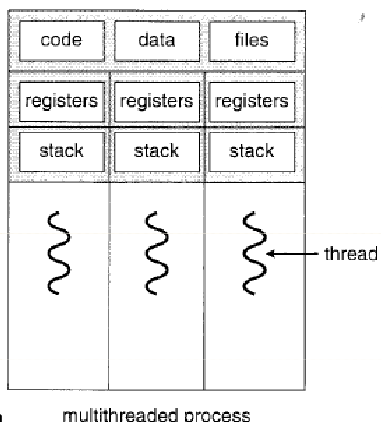
\includegraphics[scale=0.55]{../images/multi-threaded-process.png}
\label{processthread}
\end{center}
\end{figure}
\subsection{Multi-Threading Models}
The operating system will facilitate user programs via {\bf user threads} and will also facilitate concurrency in kernel space by supporting and managing {\bf kernel threads}. There must exist some mapping between the user threads and the kernel threads.
\subsubsection{Many-to-One}
In this scenario many threads are mapped to one kernel thread. This makes it particularly easy to manage threads at the application layer. The cost of switching between threads in the application layer is reduced further, since the switch is a soft one. The downside of this approach is that if two of the user threads make a blocking kernel thread call, we end up with blocking across the whole application. GNU portable threads are an example of a library that takes this approach.  
\subsubsection{One-to-One}
A more common approach is an explicit mapping between a user thread and a kernel thread. This allows multiple threads to execute in parallel on different processors, and allows a greater degree of concurrency at the application layer by not exposing these threads to blocks that are caused by the other application layers. In a typical windows application, a common use case is to display an animated message on the screen while a file is loading. In the previous case, the file I/O would block the single kernel thread and we could not show anything. In this case, we can execute concurrently. On a single processor system, the animated messages' processing is interleaved with the I/O wait quite efficiently. In the dual core approach they may be really executed in parallel to some degree. The downside to this approach is cost. Due to the common use case I just described, you will find that operating systems such as Windows and Linux can be configured to take this approach. 
\subsubsection{Many-to-Many}
Some operating systems provide a hybrid approach whereby a pool of kernel threads is maintained, and the user threads are mapped on an as-needed basis. The idea here is to multiplex onto a smaller number of kernel threads in order to manage down somewhat the overhead exhibited by the one-to-one mapping. At the same time, this approach mitigates against inter thread blocking to some degree. This degree is configurable and related to the size of the kernel thread pool. As the thread pool increases in size, the cost of management of these threads increases. HP-UX is an operating system that will take this approach. This is typically deployed in server environments that have less requirements on responsiveness but greater requirements on throughput and CPU utilization. 
\subsection{Libraries}
There are a number of common libraries that provide an API for the creation and management of threads. Some of these libraries will exist only in user space, but are more typically supplemented by kernel level support. At the system level, these libraries can be quite complex. Some threading libraries, such as the Java language threading libraries, will attempt to abstract away the complexity of the system level libraries somewhat by wrapping a subset of its functionality and exposing it as another API. Figures \ref{pthread_sum} and \ref{linux_sum} illustrate this with two small programs to sum integers in parallel. 
\begin{figure}
\caption{Linux pThreads Summation \cite{OSCONCEPTS}}
\begin{center}
\lstinputlisting[language=c]{../listings/pthread_sum.c}
\label{pthread_sum}
\end{center}
\end{figure}
\begin{figure}
\caption{Java Threads Summation. \cite{OSCONCEPTS}}
\begin{center}
\lstinputlisting[language=java]{../listings/java_sum.java}
\label{linux_sum}
\end{center}
\end{figure}
\subsection{Thread Management}
There are a number of issues to consider when managing threads that are somewhat analogous to the management of processes. 
\subsubsection{Thread Creation}
A thread creation  must only happen by means of a fork that will {\bf duplicate the creating thread only}. An execution of the {\bf exec} system call will not only duplicate the calling thread but the entire process, including any other threads that exist in the calling application. 
\subsubsection{Thread Cancellation}
A thread must either terminate itself, or be terminated by some other thread. When termination of a thread is requested it can be executed {\bf asynchronously} whereby the OS does not wait around for the thread to terminate gracefully. Alternatively, {\bf deferred cancellation} causes the operating system to periodically check if the thread is ready for termination, usually giving it warning and the opportunity to cancel itself. Graceful cancellation by the thread assists in the effective reclamation of resources, state and shared memory. In a forced termination, these are all executed immediately. If the thread to be executed has not {\bf checkpointed} it's state, that state will be lost giving in unpredictable results.  
\subsubsection{Signal Handling}
A signal, or event handler, is code that gets executed when the OS, program or user tries to communicate with the thread. The OS is responsible for the guarantee of delivery. There are synchronous signal handlers that require immediate action. Examples of such are illegal memory access, errors such as division by zero. Asynchronous signals do not require immediate handling, but there may be a time period after which an asynchronous signal will become a synchronous one. The most common example is the user action {\bf ctrl+c} which forces a process to exit. A default signal handler will almost always be provided by the underlying library. We will only replace this handler if we require special behaviour to occur as the signal is handled.   
\subsubsection{Thread Pools}
As the number of threads increases, the cost of managing these threads also increases. This may not necessarily be a linear function. At some point the presence of huge amounts of threads on a system causes so much context switching that it would be better to execute in a single threaded fashion. Furthermore, there is a cost to creating a new thread. So much so that it may not be enough to simply create these threads on demand. For these two reasons thread pools are created by both the operating system and the user applications. They are typically initialized in bulk as an up-front cost and are set to a fixed, or semi-fixed size. These pools sit idle until they are given work. When the pool has been exhausted, either the request for a new thread fails due to lack of resources, or some space in the pool is freed up. When there is a free thread in the pool and a new thread is requested, a thread in  the pool is immediately assigned some work. This can have a positive effect on the response time of the request. Web Servers will sit around with thread pools that are waiting to handle requests for web pages from users. Since for every request we do not have to create new threads, the user experience is significantly improved. Tuning thread pools in terms of size is often an empirical process. Designing your application to leverage thread pools is more of an architectural decision.
\subsubsection{Thread Specific Data}
Threads my need their own copies of data that may be duplicated in the shared memory space or may be totally scoped locally to the thread. This in particular allows partial results of work on threads to be stored before they are ready for sharing with other threads. The Java {\bf ThreadLocal } class facilitates this behaviour. It provides an area for Threads to store standard variables, with the caveat that each time a thread will store a particular value named by a key, a unique copy of the data is created that is exclusively accessable by the thread \cite{threadlocal}. A good use of this facility is in situations where you need to share state across the thread, but the state is only relevant in the context of the thread.  
\section{CPU Scheduling}
Execution of a process can be boiled down to a cycle of CPU execution, or a {\bf CPU burst} and an I/O wait followed by an {\bf I/O burst}. If a process mostly consists of CPU bursts it is CPU bound. Otherwise, if it mostly consists of I/O bursts, it is {\bf I/O bound}. CPU scheduling algorithms focus on the management of these bursts in the context of some metric. For example, our objective in any system may be to maximize the duration of CPU bursts so one important process completes without being switched out. In a time-sharing system, our priority may be to insure all process get at least a short amount of time on the CPU. The {\bf scheduler} is responsible for the selection of processes on the ready queue that should be executed. The unit of data in this queue is the process control block. 
\newline\newline
A CPU scheduling decision is required when 
\begin{itemize}
\item A process switches from running to waiting state. 
\item A process switches from running to the ready state. 
\item A process switches from the waiting state to the ready state. 
\item A process terminates. 
\end{itemize}
\subsection{Pre-Emptive Scheduling}
If a {\bf non pre-emptive} or {\bf co-operative} scheduling algorithm is used, a process can grab the CPU and release it when it is finished. This is only applicable to scenarios 1 and 4 above. Potential pitfalls of this approach are obvious, especially in a multi-programmed system such as a desktop operating system. Relying on the good nature of any programmer to release any resource, let alone the CPU, is a bad strategy. {\bf Pre-emptive} scheduling assists us here. Using a timer and some OS logic, a process is forced to give up the CPU if certain criteria are met. These are more often than not related to the executing time, or estimated execution time of the process. Interrupts facilitated this context switch. Code that is executing in Kernel space may be able to disable pre-emptive scheduling. This is particularly useful if it is imperative the kernel level call is not switched out mid-execution. 
\newline\newline
At the application layer, switching out and in processes while accessing shared data is a particularly dangerous operation. Care must be taken to ensure that results of modifications to shared state are consistent. This is a tricky problem in the general case, so the best the operating system can do is provide some features that enable application programmers to ensure shared state is consistent across switches. We will talk about this in much more detail in the next chapter. 
\subsection{The Dispatcher}
While the scheduler is responsible for choosing what process has control, the dispatcher is responsible for actually providing the control. Responsibilities of the dispatcher include 
\begin{itemize}
\item Switching Context - Loading and saving the contents of register state. 
\item Switching User Modes 
\item Affecting the PC with the correct instruction pointer
\end{itemize}
The {\bf dispatch latency} is the time taken for the dispatcher to stop one process and start another process. 
\subsection{Scheduling Criteria}
Keeping the CPU utilized, or as busy as possible is a common criterion, in particular for batch processing systems. The {\bf throughput} is defined as the number of processes executed per unit time and is important in batch processing systems such as bank transaction processors. {\bf Turnaround time} is the time from the submission of the process to the completion of the process and may be important in systems that process real-time data. The {\bf waiting time} is the sum of the periods the process spends in the waiting queue. Finally, the {\bf response time} is the time it takes to start responding to user interaction. 
\newline\newline
Our objective may be a function of all of the above criteria. Maximization of throughput and utilization go hand in hand. Minimization of turnaround time, waiting time and response time are all desirable in systems that interact with users in real-time. At a slight angle to these criteria is {\bf minimization of variance} of metrics related to all of the above criteria. This improves the predictability of a system. 
\subsection{FCFS - First Come First Served}
This is the simplest approach to scheduling. It is a {\bf non pre-emptive} algorithm in which the first process to request the CPU aquires it until it has finishing executing. Average waiting time can be quite long for this scheduling algorithm, therefore affecting both throughput and turnaround time. The CPU and device utilization characteristics are also poor due to the {\bf convoy effect}. This happens when a long running process blocks the CPU for a large period of time, and several other processes need to use this process for just a short period of time. If the long running process is waiting on I/O then the shorter processes, which may not be I/O bound, simply have to wait in line for this process to finish and release. This approach is certainly not recommended for time sharing systems.  
\begin{figure}
\caption{First Come First Served. \cite{OSCONCEPTS}}
\begin{center}
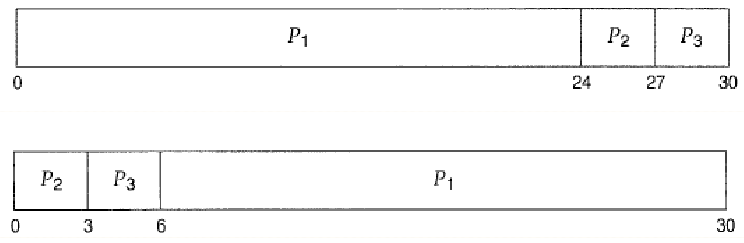
\includegraphics[scale=0.45]{../images/fcfs-sched.png}
\label{fcfs}
\end{center}
\end{figure}
\subsection{SJF - Shortest Job First}
In this algorithm, the CPU is given to the process that has the smallest next CPU burst. In the case of equality, this reduces to first-come-first-served. This gives the minimal average waiting time for a given set of processes and is provably optimal for this criterion. However, knowing the length of the next CPU cycle can be extremely difficult. At the CPU level, the only information that is useful in predicting the burst size is an exponential average over the most recent information available to the processor given past executions. This algorithm can be implemented either pre-emptively or in a non pre-emptive fashion. In the former case, when a burst has exceeded the predicted burst size, it may be placed back onto the ready queue, or it may be simply terminated. The estimated time remaining will count in this circumstance, and the algorithm is referred to a shortest time remaining algorithm.  
\begin{figure}
\caption{Shortest Job First \cite{OSCONCEPTS}}
\begin{center}
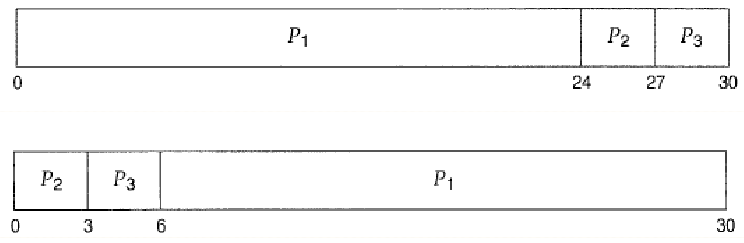
\includegraphics[scale=0.45]{../images/fcfs-sched.png}
\label{fcfs}
\end{center}
\end{figure}
\subsection{RRS - Round Robin Scheduling}
In this algorithm, a time slice is defined, usually in the 10ms to 100ms range. The ready queue is a circular FIFO queue, such as a ring-buffer. A process will be given its time-slice to do some work and will be switched off the CPU once this time slice has expired. This is fully a pre-emptive scheduling algorithm. Average waiting time can be long with this algorithm, and typically the size of the time slice is the single biggest factor in determining if this is true. When round-robin scheduling, the number of context switches executed by the dispatcher is sensitive. As a general rule of thumb, the time slice should be picked to be short enough that 80 percent of CPU burst are shorter than it. This keeps the queues of a manageable size, the turnaround time acceptable while ensuring context switches are not too much of a factor. 
\begin{figure}
\caption{Round Robin Scheduling \cite{OSCONCEPTS}}
\begin{center}
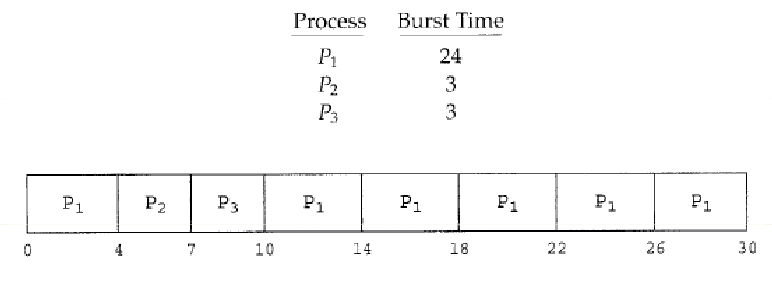
\includegraphics[scale=0.45]{../images/rr-sched.png}
\label{fcfs}
\end{center}
\end{figure}
\subsection{Multi-Level Queue Scheduling}
When processes can be classified into groups with differing scheduling characteristics, using multi-level queues becomes useful. The commonest division is when processes are classed as either {\bf background} or {\bf foreground}. These differ in requirements on turnaround time and response time. With multi-level scheduling, the ready queue is partitioned into several separate queues. At each level, a different algorithm may be applied. To ensure that {\bf starvation} is minimized, we may include a feedback mechanism. If a background process is waiting in a queue division for too long it may be promoted into the foreground automatically. Similarly, a foreground process may decay into a background class process over time. Figure \ref{mlq} illustrates this. 
\begin{figure}
\caption{Multi-Level Scheduling with Feedback \cite{OSCONCEPTS}}
\begin{center}
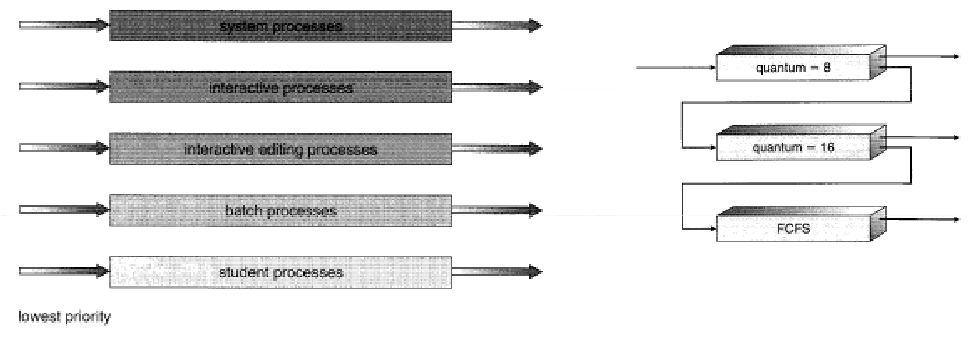
\includegraphics[scale=0.36]{../images/ml-sched.png}
\label{mlq}
\end{center}
\end{figure}
\subsection{Multi-Processor Scheduling}
On multi processor systems, we may have {\bf asymmetric} multi-processing or {\bf symmetric multiprocessing}. In the former case, one processor is the master and its scheduler is responsible for farming jobs out to different slave CPUs. In the symmetric case, each processor is self scheduling. There can be a high cost in moving processes between assigned CPUs after execution is started. A process will typically have an {\bf affinity} for one CPU once it begins. This guarantee may be a soft - i.e. best effort - or a hard guarantee. 
\newline\newline
{\bf Load Balancing} attempts to keep workload evenly distributed across processors. Each processor necessarily has its own ready queue and a load balancer may invoke {\bf push migration} where it moves work away from processors that are too busy by some measure. Conversely, the CPU scheduler may invoke {\bf pull migration} where an idle scheduler fills its empty queue with jobs from another processor.
\subsection{Thread Scheduling}
The {\bf process contention scope} is where user threads vie with each other to be mapped onto kernel threads. This is facilitated by an LWP or {\bf lightweight process}. It is actually at the {\bf system contention scope} where CPU scheduling takes place, and it is kernel threads that are  scheduled on the CPU. 
\subsection{Windows XP}
Windows XP exhibits priority based, time-sliced pre-emptive scheduling. A thread will run on a CPU until either a blocking system call, it terminates or until the end of its time quantum. It provides a 32 level priority scheme to associate priorities with various threads. In this regard, multi-level scheduling is used. Some feedback is implemented, in that foreground processes that are moved from the background are automatically promoted in priority when they are selected by the user. There is one queue per scheduling priority. The {\bf idle thread} is executed if there is nothing to do. Figure \ref{xpched} shows the priority matrix in detail. 
\begin{figure}
\caption{Windows XP Thread Priorities \cite{OSCONCEPTS}}
\begin{center}
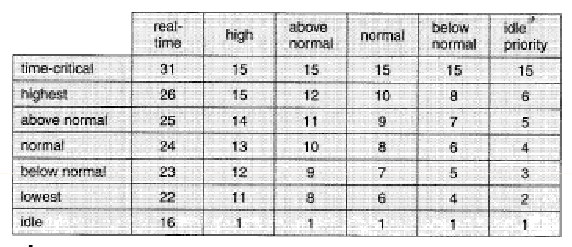
\includegraphics[scale=0.45]{../images/xp-sched.png}
\label{xpched}
\end{center}
\end{figure}
\subsection{Linux}
Linux uses a pre-emptive, priority based algorithm with two separate priority ranges. The time quantum is variable and related to the priority of a process. The classes are {\bf realtime} and {\bf nice}. A process is eligible for execution when it has not exhausted its time-slice. Thereafter it must wait for other processes to exhaust theirs before it receives a new time-slice. Each processor has its own {\bf run-queue} which tracks an {\bf active} and {\bf expired} priority array. Real-time tasks have static priorities, while others have a dynamic priority based on their nice values.  The nice value is adjusted in a range from 100 to 140 based on how long a task has been sleeping for I/O. The nice value is adjusted to favour interactive tasks that conduct lots of I/O. CPU priorities have far shorter sleep times, but they also have lower priorities. 

\bibliography{../biblio/techfundamentals.bib}{}
\bibliographystyle{plain}
\begin{center}
{\small \copyright  David Lynch 2012. Do not reproduce without written permission.}
\end{center}
\end{document}
